This chapter guides you through the features of MongoDB. Whereby we go through what is MongoDB in general, Data model and CRUD Principles. Thereafter we check through the Use-Cases of MongoDB and performance and limitations. Additionally, we get a short Insight how MongoDB is used in a Big Data context. After all, we come up with a conclusion.

\section{What is MongoDB ?}
MongoDB is a part of NoSQL family and belongs to the document-oriented databases. Therefore, it doesn’t have the concepts of tables, rows and columns. Instead, MongoDB is built on an architecture of collections and documents. Documents contain sets of key- value pairs like JSON and are the basic unit of data in MongoDB. A collection includes a set of documents and offers the same functionality as relational database tables\cite{Banker2016}
\begin{figure}[H]
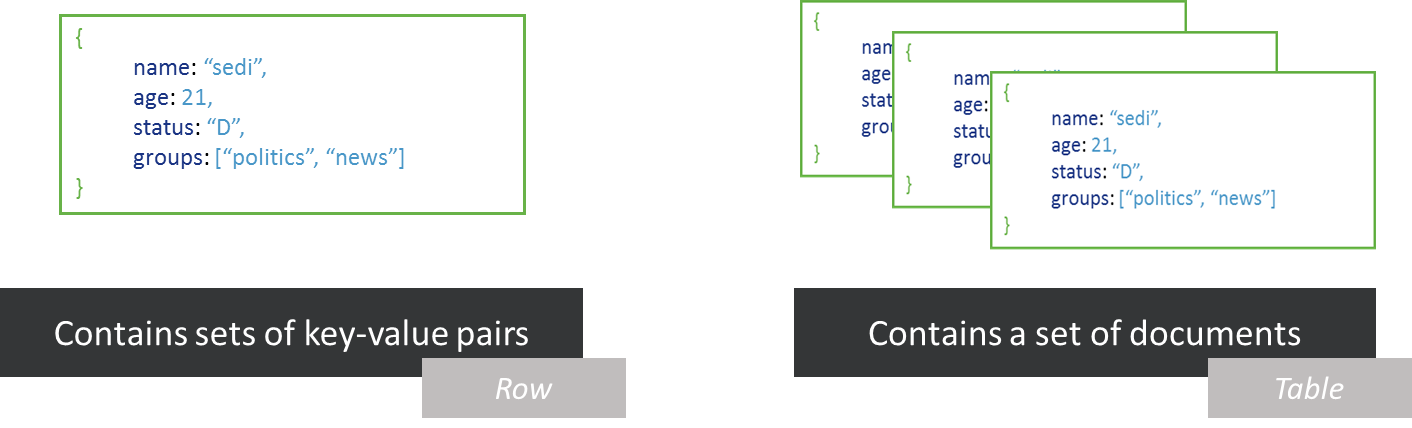
\includegraphics[width=\linewidth,keepaspectratio]{images/documentscollections.png}
\caption{Documents and collections}
\end{figure}

MongoDB stores data as Binary JSON documents also known as BSON. The documents can have different schemas, which means that the schema can change dynamically as the application evolves. Automatic sharding enables data in a collection to be distributed across multiple systems for horizontal scalability as data volumes increase\cite{Edward2015}. Additional, MongoDB doesn’t only support Key-Value operations. It allows complex queries, aggregations and secondary indexes that unlock the value in structured, semi-structured and unstructured data. One of MongoDB’s major features is the support for many types of queries like text search, range queries, geospatial queries over to MapReduce queries\cite{MongoDBInc.2013a}.
\\
MongoDB was created by Dwight Merriman and Eliot Horowitz, who had encountered development and scalability issues with traditional relational database approaches while building Web applications at DoubleClick, an Internet advertising company that is now owned by Google Inc. The database was released to open source in 2009 and is available under the terms of the Free Software Foundation's GNU AGPL Version 3.0 commercial license. However, the database is one of the most popular NoSQL databases and is used by several company like Bosch, Facebook, Expedia and so on\cite{Hows2013}.

\section{Use Cases: What is MongoDB for?}
This section will give you an insight between the features and potential of MongoDB and some problems that is suited to solve.
\\
Beginning with online and mobile Apps. Nowadays Companies want their business on their smartphones or access it from everywhere through the web. In comparison to RDMBS MongoDB addresses the upcoming challenges of these plans. Furthermore, MongoDB promises to make it easier than other alternatives. Requirements for going mobile or online are hard to manage. For example, different types of device like smartphone or wearables are creating new types of unstructured and semi-structured data. Another reason is the number of devices and users. Meanwhile, Response times must keep and provide the same User experience. So, Scalability has now a high priority. MongoDB tries to decrease the degree of difficulty for these Requirements. That is why MongoDB offers a flexible data model and rich query functionality. Therefore, MongoDB can manage any kind of data, no matter how dynamically the data changes. In addition to that, MongoDB’s development concentrates on scalability and can handle a lot of Users and data sets\cite{MongoDBInc.2013a}.
\\
Another Example for a suited use case is a catalog. Mention that almost anybody knows some requirements a Catalog must meet. Deleting, creating and changing items or their features or their attributes – only to mention few - are a standard set of Requirement of a catalog. Behind the scenes, we see a lot of challenges for a RDMS. There will be a lot of changes in the data, like new data and new metadata to your catalogs. We already talked about the untrusted and semi-structured in the first Use case. Again, we got the same problems with a RDBMS. How does MongoDB make it easier for developers? First, it is how the data is structured in MongoDB. With MongoDB’s JSON document model makes it easy to store different assets with different attributes in a single place. It also makes it simple to represent complex, hierarchical relationships. Schemas in MongoDB are self-describing. You can add new products and features and evolve the schema instantly, without taking the database down or impacting performance. Lastly an expressive query language, indexing, including text search and geospatial, and analytics provide flexible access to the data, no matter how the application, business or developer needs to find it\cite{MongoDBInc.2013a}.
\\
All in all, these are only few examples for use cases and for what MongoDB is. In general MongoDB claims to be suited for high flexible data schemas to provide the ability for data changes, structed, unstructured and semi structured data. Additionally, MongoDB eco system let developer spend less time for the design of models, entities, relationships and tables, and more time on the application\cite{MongoDBInc.2013a}.
